\documentclass[a4paper,12pt]{article}
\usepackage{HomeWorkTemplate}

\usepackage[utf8]{inputenc}
\usepackage[]{babel}

\setlength{\parindent}{4em}
\setlength{\parskip}{0.5em}

\renewcommand{\baselinestretch}{1.5}


\usepackage{caption}
\usepackage{subcaption}
\usepackage{graphicx}
\usepackage{float}
\usepackage[utf8]{inputenc}
\usepackage{lmodern, textcomp}
\usepackage{circuitikz}
\usepackage[shortlabels]{enumitem}
\usepackage{hyperref}
\usepackage{tikz}
\usepackage{amsmath}
\usepackage{amssymb}
\usepackage{tcolorbox}
\usepackage{graphicx}
\usepackage{xepersian}
\settextfont{XB Niloofar}
\usetikzlibrary{arrows,automata}
\usetikzlibrary{circuits.logic.US}
\usepackage{changepage}
\newcounter{problemcounter}
\newcounter{subproblemcounter}
\setcounter{problemcounter}{1}
\setcounter{subproblemcounter}{1}
\newcommand{\problem}[1]
{
	\subsection*{
		پرسش
		\arabic{problemcounter} 
		\stepcounter{problemcounter}
		\setcounter{subproblemcounter}{1}
		#1
	}
}
\newcommand{\subproblem}{
	\textbf{\harfi{subproblemcounter})}\stepcounter{subproblemcounter}
}


\begin{document}
	\handout
	{اصول پردازش تصویر}
	{دکتر مصطفی کمالی تبریزی}
	{نیم‌سال اول 1399\lr{-}1400}
	{اطلاعیه}
	{سیدعلیرضا خادم}
	{97100398}
	{تمرین سری پنجم - سوال دوم}
	زمان حدودی اجرا: کمتر از 5 ثانیه 
	
	ابعاد تصویر
	\lr{apple}:
	$ 512{px} \times 512{px} $
	
	ابعاد تصویر
	\lr{orange}:
	$ 512{px} \times 512{px} $
	
	\section*{موارد لازم.}
	برای اجرا لازم است تا تصاویر 
	\lr{apple.jpg}
	و
	\lr{orange.jpg}
	در مسیر
	\lr{EX5\_Q2/}
	قرار داشته باشد. همچنین در پیاده‌سازی این سوال از کتابخانه‌های 
	\lr{cv2}
	و
	\lr{numpy}
	استفاده شده است که قبل از اجرا بایستی این کتابخانه‌ها روی سیستم شما نصب باشد.
	\section*{روند کلی حل.}
	ایده کلی حل این سوال استفاده از هرم‌های 
	\lr{laplacian}
	و 
	\lr{gaussian}
	برای 
	\lr{blendig}
	است. 
	\begin{figure}[H]
		\centering
		\begin{subfigure}{0.9\textwidth}
			\centering
			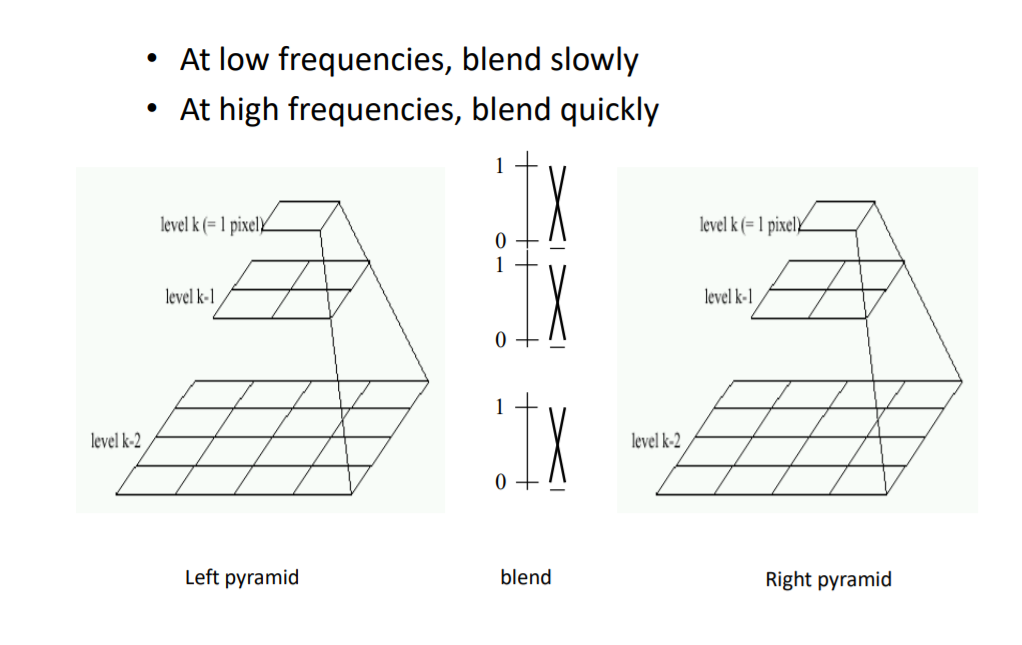
\includegraphics[width=.8\textwidth]{2.png}
		\end{subfigure}
	\end{figure}
	در این روش ابتدا برای دو تصویر 
	\lr{laplacian pyramid}
	را به دست ‌می‌آوریم، و برای 
	\lr{mask}
	هم 
	\lr{gaussian pyramid}
	را به دست می‌آوریم. در ادامه هر سطح از هرم را با استفاده از سطح متناظرِ
	\lr{mask}
	از 
	\lr{gaussian pyramid}‌یِ
	آن ترکیب می‌کنیم. (با توجه به رابطه‌ای که در ادامه آمده است.)
	\begin{figure}[H]
		\centering
		\begin{subfigure}{0.9\textwidth}
			\centering
			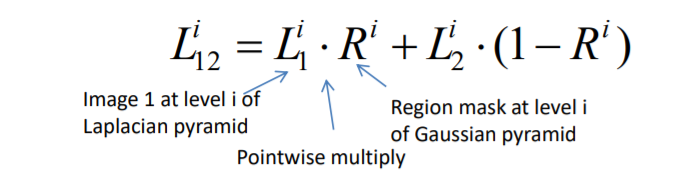
\includegraphics[width=\textwidth]{1.png}
		\end{subfigure}
	\end{figure}
	کلیت پیاده‌سازی الگوریتم هم در ادامه آمده است.
	\begin{figure}[H]
		\centering
		\begin{subfigure}{0.9\textwidth}
			\centering
			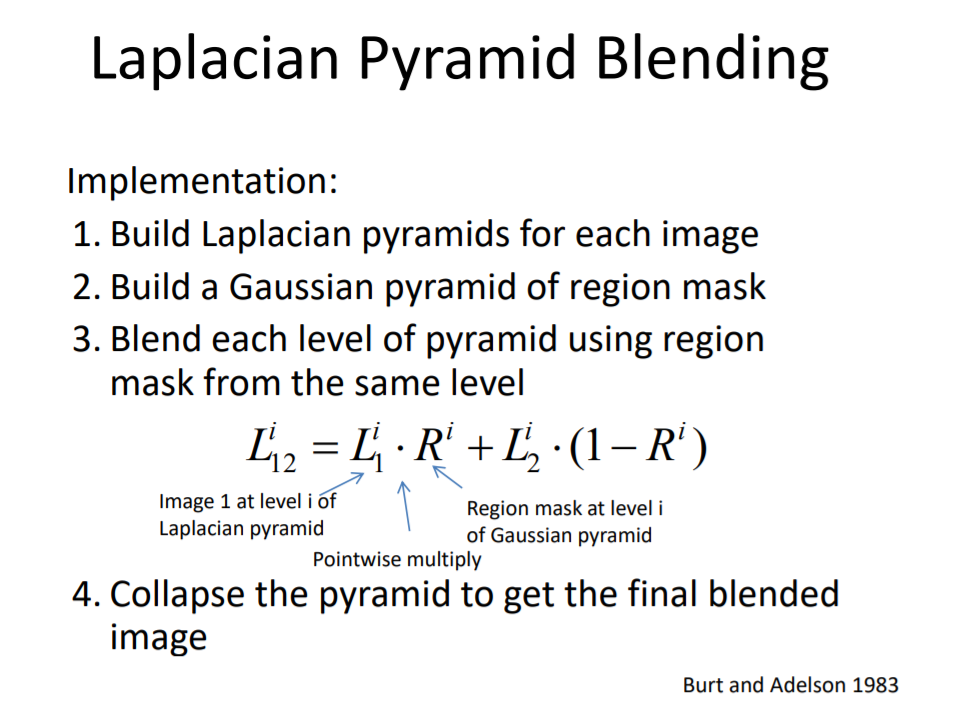
\includegraphics[width=\textwidth]{3.png}
		\end{subfigure}
	\end{figure}
	
	
	
	\section*{توضیح کد.}
	برنامه در مجموع حاوی 2 فایل با فرمت
	\lr{.py}
	می‌باشد که توضیحات هر فایل در پایین آمده است.
	\subsection*{$\circ$ utilities.py}
	\subsubsection*{\lr{get\_gaussian\_pyramid(src\_image, num\_levels)}}
	این تابع یک تصویر و یک عدد را به عنوان ورودی می‌گیرد و هرم 
	\lr{gaussian}
	مربوط به 
	\lr{src\_image}
	با 
	\lr{num\_levels}
	سطح خروجی می‌دهد.
	\subsubsection*{\lr{get\_laplacian\_pyramid(src\_image, num\_levels)}}
	این تابع یک تصویر و یک عدد را به عنوان ورودی می‌گیرد و هرم 
	\lr{laplacian}
	مربوط به 
	\lr{src\_image}
	با 
	\lr{num\_levels}
	سطح خروجی می‌دهد.
	\subsubsection*{\lr{get\_blended\_pyramid(lp\_source, lp\_target, gp\_mask)}}
	این تابع هرمِ 
	\lr{laplacian}ِ
	تصویرِ
	\lr{source}
	،
	هرمِ
	\lr{laplacian}ِ
	تصویرِ
	\lr{target}
	و
	 هرمِ
	 \lr{gaussian}ِ
	 تصویرِ
	 \lr{mask}
	 را به عنوان ورودی می‌گیرد و 
	 \lr{blended\_pyramid}
	 را با توجه به روابط زیر ساخته به به عنوان خروجی بر‌می‌گرداند.
	 \begin{figure}[H]
	 	\centering
	 	\begin{subfigure}{0.9\textwidth}
	 		\centering
	 		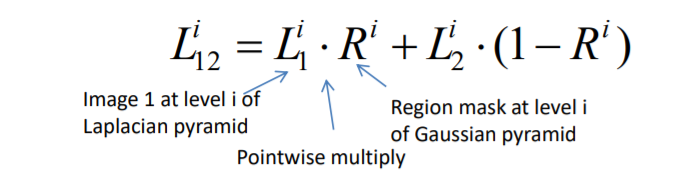
\includegraphics[width=\textwidth]{1.png}
	 	\end{subfigure}
	 \end{figure}
 \subsubsection*{\lr{reconstruct\_channel(blended\_pyramid)}}
	 این تابع 
	 \lr{blended\_pyramid}
	 را به عنوان ورودی می‌گیرد و با استفاده از تابع
	 \lr{cv2.pyrUP}
	 عملیات 
	 \lr{collapse}
	 را انجام می‌دهد.
	\subsubsection*{\lr{blend\_channel(source\_channel, target\_channel, mask)}}
	این تابع یک کانال از تصویر
	\lr{source}
	و یک کانال از تصویر
	\lr{target}
	را به همراه 
	\lr{mask}
	به عنوان ورودی می‌گیرد و با استفاده از توابع 
	\lr{get\_blended\_pyramid}
	و
	\lr{reconstruct\_channel}
	این دو چنل را با هم ترکیب کرده و نتیجه را به عنوان خروجی بر‌می‌گرداند.
	\subsubsection*{\lr{pyramid\_blend(source, target, mask)}}
	این تابع تصاویر 
	\lr{sourcr}
	،
	\lr{target}
	و
	\lr{mask}
	را به عنوان ورودی می‌گیرد و با استفاده از تابع 
	\lr{blend\_channel}
	برای هر یک از کانال‌های تصاویر، به صورت مجزا 
	\lr{blending}
	را انجام می‌دهد و تصویر حاصل را به عنوان خروجی بر‌می‌گرداند.
	\subsubsection*{\lr{mouse\_handler}}
	این تابع رویدادهای مربوط به 
	\lr{mouse}
	را مدیریت می‌کند تا کاربر بتواند رئوسِ چندوجهی 
	\lr{mask}
	را ورودی دهد.
	\subsubsection*{\lr{get\_mask(shape, vertices)}}
	این تابع رئوس و ابعاد 
	\lr{mask}
	را ورودی می‌گیرد و با استفاده از تابع 
	\lr{fillConvexPoly}
	،
	\lr{mask}
	را می‌سازد و به عنوان خروجی بر‌می‌گرداند.
	\subsection*{$\circ$ q2.py}
	در این فایل ابتدا تصاویر را لود می‌کند و در ادامه تصویر
	\lr{apple\_image}
	برای کابر نمایش داده می‌شود تا راس‌های چندوجهیِ
	\lr{mask}
	را با کلیک چپ روی تصویر مشخص کند. منتظر می‌ماند تا کاربر بعد از وارد کردن راس‌ها،
	دکمه 
	\lr{ESC}
	از کیبرد را بفشارد. بعد از فشرده‌شدن دکمه 
	\lr{ECS}
	توسط کابر، با توجه به رئوسی که کابر وارد کرده 
	\lr{mask}
	ساخته می‌شود. درنهایت با فراخوانی تابع 
	\lr{pyramid\_blend}
	روی ورودی‌هایی که مشاهده می‌کنید،
	\lr{result}
	را محاسبه می‌کند و با نام 
	\lr{res2.jpg}
	در مسیر 
	\lr{EX5\_Q2/results}
	ذخیره می‌کند.
\end{document}
